\chapter{Related Works} \label{chapt:RelatedWorks}

Association discovery \cite{arm1} is one of the most researched topics in data mining. However, the fielded applications appear to be relatively few, especially for applying association rule mining techniques to data streams, which becomes more common in real-world scenarios.

It has been suggested that this is due to the susceptibility of conventional association discovery techniques to finding large numbers of associations that are unlikely to be interesting to the user \cite{topk}. In this chapter I will survey and summarise the literature of association rule mining and how to detect and adapt to the concept drifts.

The structure of this chapter is as follows. Section \ref{sec:2.1} discusses basic knowledge of data streams. Section \ref{sec:2.2} discusses the preliminaries on association rule mining and some mainstream association rule mining techniques. Section \ref{sec:2.3} discusses basics of concept drift and several popular drift detectors. Section \ref{sec:2.4} explains the definition of self-sufficient itemset and why we adopted it in our proposed framework. Section \ref{sec:2.5} summarises this section.


\section{Data Stream Basics}\label{sec:2.1}
In this section, several basic definitions of data stream will be discussed first, followed by discussing the current general processing approaches.

A data stream is a sequence of data instances arriving continuously. It is considered to be dynamic and unbounded in size with data generated at a very fast pace. Generally, a dynamic data stream cannot be processed in the same way as a static database. Dynamic data streams requires one-pass techniques using either batch processing or online processing of data.

In this dissertation, our concentration is transactional data stream which consists infinite number of transactions.

%\theoremstyle{definition}
%\begin{definition}{Data Stream}
\begin{definition}[\textbf{\textit{Transactional Data Stream}}]
\label{datastream}
A data stream $\mathcal{D}$ with $n$ elements is defined as $\mathcal{D} = \{T_1, T_2, ..., T_n\}$, where by $T_i$ represents a transaction at time $i$. Each transaction contains a set of items $T = \{x_1, x_2, \ldots x_m\}$, where by $x_j$ represents an item. 
\end{definition}

Next, we will review the the mainstream processing approaches of data stream.

\subsection{Processing Approaches}
Due to the constraints of data streams: one-time access, continuous processing, limited memory, and fast response, data stream processing needs to be very efficient and computationally affordable. There are a number of different streaming methods proposed for data streams but there are two approaches that are predominantly considered: batch processing approach and sliding-window approach. Read et al. \cite{ds} provides a comparison of processing approaches in data streams.

\subsubsection{Batch processing approach}
Batch processing divides data stream into batches, different batches will be fed into mining techniques to solve tasks. The batch generation criteria can be time on how long data will be collected before dispatching processing on it or a fixed interval on data stream. 

\begin{figure}[H]
    \centering
    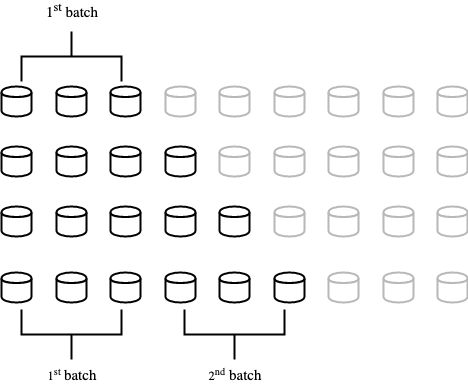
\includegraphics[width=0.6\textwidth]{RelatedWorks/batch.png}
    \caption{An example of batch processing approach}
    \label{fig:abrupt}
\end{figure}

\subsubsection{Sliding-window approach}
In the sliding window approach, data is processed after
the arrival of every single data instance. A sliding window generally has a fixed size and data is kept in the window based on the first in first out (FIFO) rule. The window moves when new data instance arrives, it slides to store the new data by dropping the oldest instance in the window, which keeps data in the window updated at any time point.

\begin{figure}[H]
    \centering
    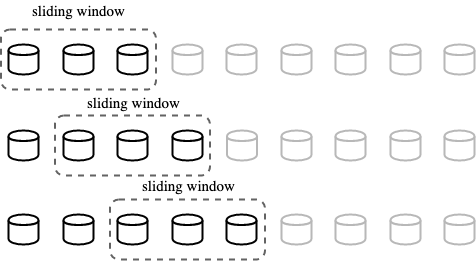
\includegraphics[width=0.6\textwidth]{RelatedWorks/window.png}
    \caption{An example of sliding-window approach}
    \label{fig:abrupt}
\end{figure}

\section{Association Rules} \label{sec:2.2}
To discover interesting patterns and relationships in data streams, association rules mining plays a key role in mining data streams. Firstly, the definition of frequent itemsets is introduced to help understand and create association rules.

\begin{definition}[\textbf{\textit{Frequent Itemset}}]
\label{freqitemset}
Frequent itemset, as it appears to mean, is itemset which appears frequently in a data stream. To determine if an itemset is frequent or not, the definition of support value is introduced: the support of an itemset $X$ with respect to data stream $\mathcal{D}$ with $n$ transactions is defined as the proportion of transactions $T$ in the dataset which contains the itemset $X$.
\end{definition}

\[ support(X)=\frac{|T \in \mathcal{D}, X \subseteq T|}{|n|} \]

Usually, a preset minimum support threshold is used to determine if an itemset is frequent or not. Once the support of an itemset surpass the minimum support threshold, it can be determined as a frequent itemset.

Here we use a sample database in Table \ref{tb:tidlist}, it consists five transactions with seven distinct items, and the minimum support threshold is set to 2.

\begin{table}[h!]
\caption{Set of Five Transactions}
\label{tb:tidlist}
\centering
 \begin{tabular}{p{6cm}} 
 \hline\hline
 \multicolumn{1}{c}{Transactions (tid: items)}\\
 \hline
 1: a, b, c, d, e \\ 
 %\hline
 2: a, b, c, d, f, h \\
 %\hline
 3: a, f, g \\
 %\hline
 4: b, e, f, g \\
 %\hline
 5: a, b, c, d, e, h \\
 \hline
\end{tabular}
\end{table}

\begin{definition}[\textbf{\textit{Association Rules}}]
\label{ar}
Association rules are if-then statements that help to show the probability of relationships between data items within data streams. They are calculated from itemsets, which are made up of two or more items, using the measure of \textit{support}, \textit{confidence} and \textit{lift}.
\end{definition}

To mine association rules, both LHS and RHS of a rule shall come from the frequent itemsets. Here another indicator \textit{confidence} level is introduced to indicate how often the rule has been found to be true.

The confidence value of a rule, $X \Rightarrow Y$, with respect to a set of transactions $T$, is the proportion of the transactions that contains $X$ which also contains $Y$.

\[confidence(X \Rightarrow Y) = \frac{support(X \cup Y)}{support(X)}\]

Similar to frequent itemsets, when the confidence of a rule surpasses the preset minimum confidence threshold, this rule might be labelled interesting.

\subsection{Join-based Association Rule Mining Algorithms}

The most basic join-based algorithm for association rule mining is Apriori algorithm \cite{apriori}. 

\begin{definition}[\textbf{\textit{Apriori}}]
\label{Apriori}
The key concept of Apriori algorithm is the anti-monotonicity of support value, it assumes that: all subsets of a frequent itemset must be all frequent.
\end{definition}

Apriori uses a breadth-first search strategy to count the support of itemsets and uses a candidate generation function which exploits the downward closure property of support. A simple example of Apriori algorithm is shown below in Figure \ref{fig:apriori} using data from Table \ref{tb:tidlist}.

\begin{figure}[H]
    \centering
    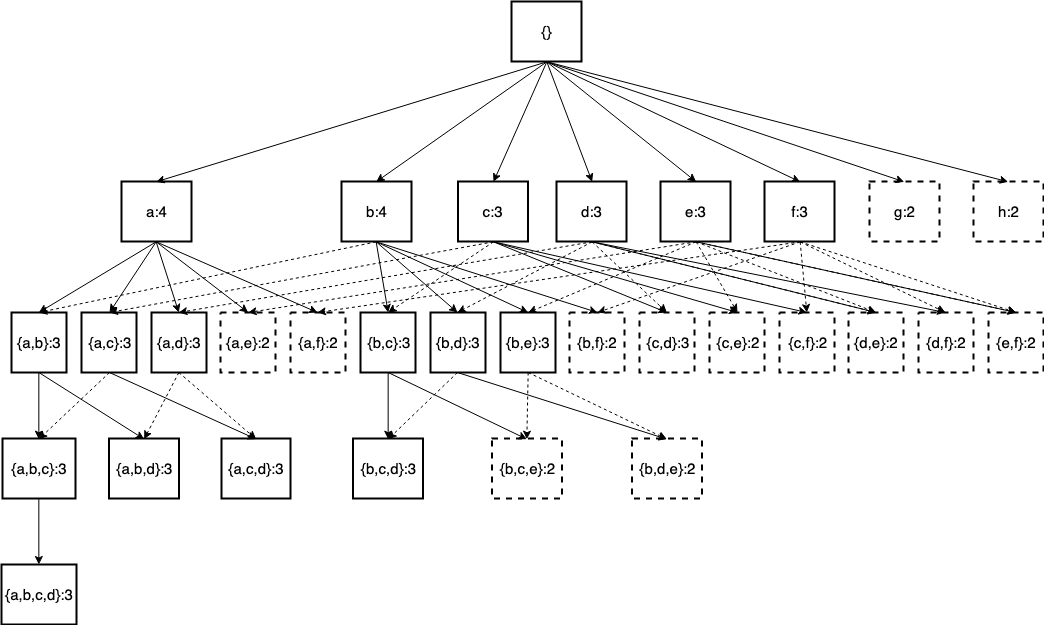
\includegraphics[width=1.0\textwidth]{RelatedWorks/apriori.png}
    \caption{An example of Apriori algorithm \cite{apriorifig}}
    \label{fig:apriori}
\end{figure}

Because of its very expensive computational cost of scanning the whole data and support counting, there are numerous optimisations proposed during the last two decades. Together with the proposal of the Apriori algorithm, Agrawal et al \cite{apriori} proposed AprioriTid and AprioriHybride as two practical optimisations. AprioriTid \cite{apriori} replaces every transaction in the database by the set of candidate itemsets that occur in that transaction, which significantly reduces the time consumed counting support values. AprioriHybrid combines Apriori and AprioriTid into a single hybrid which achieves a more flexible solution for association rule mining \cite{apriori}.

Rather than AprioriTid and AprioriHybrid, there are also other techniques proposed to optimise original Apriori algorithm, such as the work done in \cite{apriori2} and \cite{apriori3}.

To speed up the Apriori method, DHP algorithm, also known as Direct Hashing and Pruning method was proposed in 1995 \cite{DHP}.

\begin{definition}[\textbf{\textit{Direct Hashing and Pruning}}]
\label{DHP}
 There are two optimisations used in DHP \cite{DHP}. First, the candidate itemsets are going to be pruned when each new iteration happens. Second, not every whole transaction will be fed, there will be a trimming process of transactions to speed up the algorithm.
\end{definition}

To avoid meaningless itemsets when the next new candidate itemsets need to generated, DHP uses hash functions to remove them in advance. While Apriori requires to scan the entire database, which potentially massively increases the computational cost, DHP reduced the candidate itemset size. It has been proved that DHP performs significantly faster than the original Apriori algorithm.

Figure \ref{fig:dhp} below gives a simple example of how DHP works. In this case, we will not use the transactional data in Table \ref{tb:tidlist} which is going to need a very long hash table. Here we use a smaller database and perform DHP based on that. 

\begin{figure}[H]
    \centering
    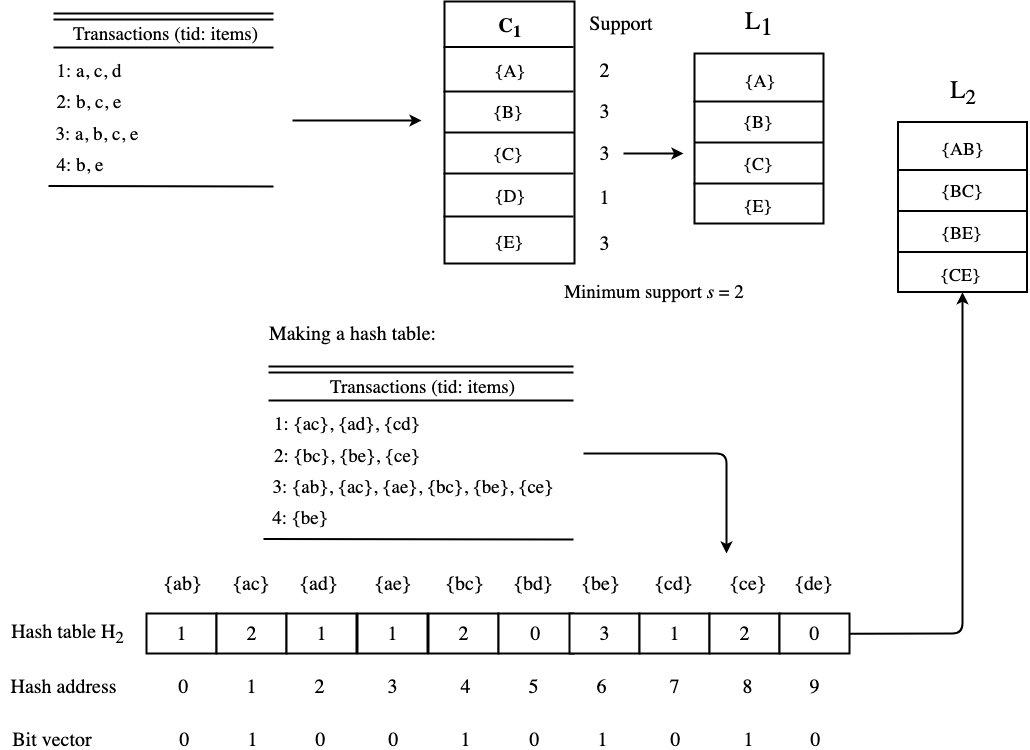
\includegraphics[width=1.0\textwidth]{RelatedWorks/DHP.png}
    \caption{An example of DHP algorithm \cite{DHP}}
    \label{fig:dhp}
\end{figure}

To reduce the computational cost of support counting in association rule mining is to find support of multiple frequent itemsets at one time. In 2004, Uno et al \cite{LCM} proposed LCM algorithm to use hyper-cube decomposition to achieve this goal. 

\begin{definition}[\textbf{\textit{LCM Algorithm}}]
\label{LCM}
The multiple itemsets obtained at the same one time, comprise a hypercube in the itemset lattice. For a frequent itemset $S$, let $H(S)$ be the set of items $a$ satisfying $a > tail(S)$ and transactions $T(S)=T(S\cup \{a\})$. Then, for any $P\subseteq H(S)$, $T(S\cup P)=T(S)$ holds, and $S\cup P$ is frequent. LCMfreq \cite{LCM} uses this property. For two itemsets $S$ and $S\cup P$, we say that $S'$ is between $S$ and $S\cup P$ if $S \subseteq S' \subseteq S \cup P$. In the iteration with respect to $S$, we output all $S'$ between $S$ and $S \cup H(S)$ \cite{LCM}.
\end{definition}

LCM saves about $2^{|H(S)|}$ times of the frequency counting \cite{LCM}.

\subsection{Tree-based Association Rule Mining Algorithms}

Another mainstream association mining technique is tree-based. They are based on set-enumeration concepts, which uses a subgraph of the lattice of itemsets to explore the candidate itemsets. Therefore, they will be used interchangeably, thus, the problem of generating frequent itemset will be constructing a enumeration tree.

\begin{definition}[\textbf{\textit{AIS Algorithm}}]
\label{AIS}
AIS algorithm was proposed by Agrawal et al \cite{arm2} in 1994, is basically a lexicographic tree algorithm. AIS constructs level-wise trees, itemsets are counting based on the transactional database with corresponding levels. AIS is a na\"ive mechanism, it searches the entire space without optimisation. 
\end{definition}

Many researchers proved that using vertical database layout could achieve significant performance improvements comparing to traditional intersection based counting techniques. Basically, for each transaction identifiers, one can have a list of items that are contained in it. And this is often referred as \textit{tidlist}. One of the earliest invention was Eclat proposed by Zaki \cite{eclat}. Here we will still use sample database in Table \ref{tb:tidlist} to illustrate the algorithms mentioned next, and the vertical representation of Table \ref{tb:tidlist} is shown in Table \ref{tb:tidlistvert} below. In this case, for instance, itemset $\{a,b\}$ can be computed as the length of the intersection of the \textit{tidlists} of $a$ and $b$.

\begin{table}[h!]
\caption{Vertical Presentation}
\label{tb:tidlistvert}
\centering
 \begin{tabular}{p{4cm}} 
 \hline\hline
 \multicolumn{1}{c}{Frequent Items (Item: \textit{tidlists})}\\
 \hline
 a: 1, 2, 3, 5 \\ 
 %\hline
 b: 1, 2, 4, 5 \\
 %\hline
 c: 1, 2, 5 \\
 %\hline
 d: 1, 2, 5 \\
 %\hline
 e: 1, 4, 5 \\
 f: 2, 3, 4\\
 g: 3, 4\\
 h: 2, 5\\
 \hline
\end{tabular}
\end{table}

\begin{definition}[\textbf{\textit{Eclat}}]
\label{eclat}
Eclat \cite{eclat} uses intersection based approach to calculate itemset support values in a vertical database. The partitioning approach is similar to Apriori algorithm \cite{apriori} but Eclat essentially generates candidate itemsets using only the join step from Apriori. 
\end{definition}

First, Eclat gets \textit{tidlist} for each item using DB scan. In this case, we use an item $a$ as an example. \textit{tidlist} of $a$ is exactly the list of transactions containing $a$. Next, Eclat intersects \textit{tidlist} of $a$ with \textit{tidlists} of all other items, resulting in \textit{tidlists} of $\{a,b\}, \{a,c\}, \{a,d\}$, which is called $a$-conditional database (removed $a$). Eclat repeats from 1 on $a$-conditional database and then repeats for all other items.

Figure \ref{fig:eclat} \cite{survey2014} illustrates the itemset generation tree with support computation by \textit{tidlist} intersection for transactions in Table \ref{tb:tidlist}.

\begin{figure}[H]
    \centering
    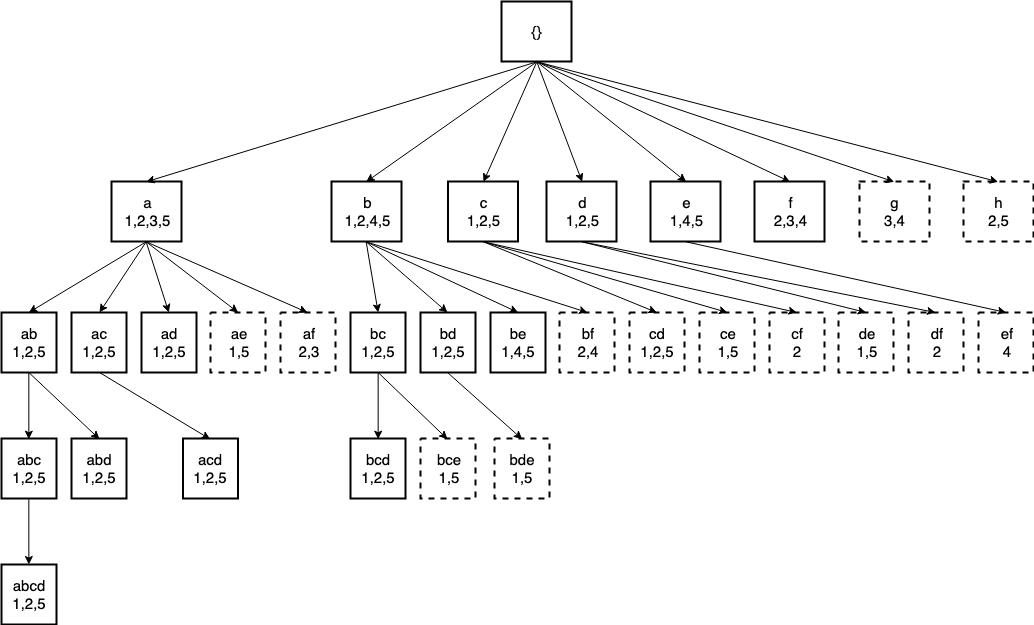
\includegraphics[width=1.0\textwidth]{RelatedWorks/eclat.png}
    \caption{An example of Eclat \cite{survey2014}}
    \label{fig:eclat}
\end{figure}

Another mainstream popular tree-based algorithm is FP-Tree. It uses compressed representations of the transactional database for more efficient counting.

\begin{definition}[\textbf{\textit{FP-Growth}}]
\label{FP}
The FP-Growth Algorithm, proposed by Han \cite{fp}, is an efficient and scalable method for mining the complete set of frequent patterns by pattern fragment growth, using an extended prefix-tree structure for storing compressed and crucial information about frequent patterns named frequent-pattern tree.
\end{definition}

In the first pass, the algorithm counts occurrence of items (attribute-value pairs) in the dataset, and stores them to 'header table'. In the second pass, it builds the FP-Tree structure by inserting instances. Items in each instance have to be sorted by descending order of their frequency in the dataset, so that the tree can be processed quickly. Items in each instance that do not meet minimum coverage threshold are discarded. If many instances share most frequent items, FP-Tree provides high compression close to tree root.

Now we can build an FP-Tree based on the support values of each distinct item in the Table \ref{tb:tidlist} which is illustrated in Figure \ref{fig:fp} \cite{survey2014}.

\begin{figure}[H]
    \centering
    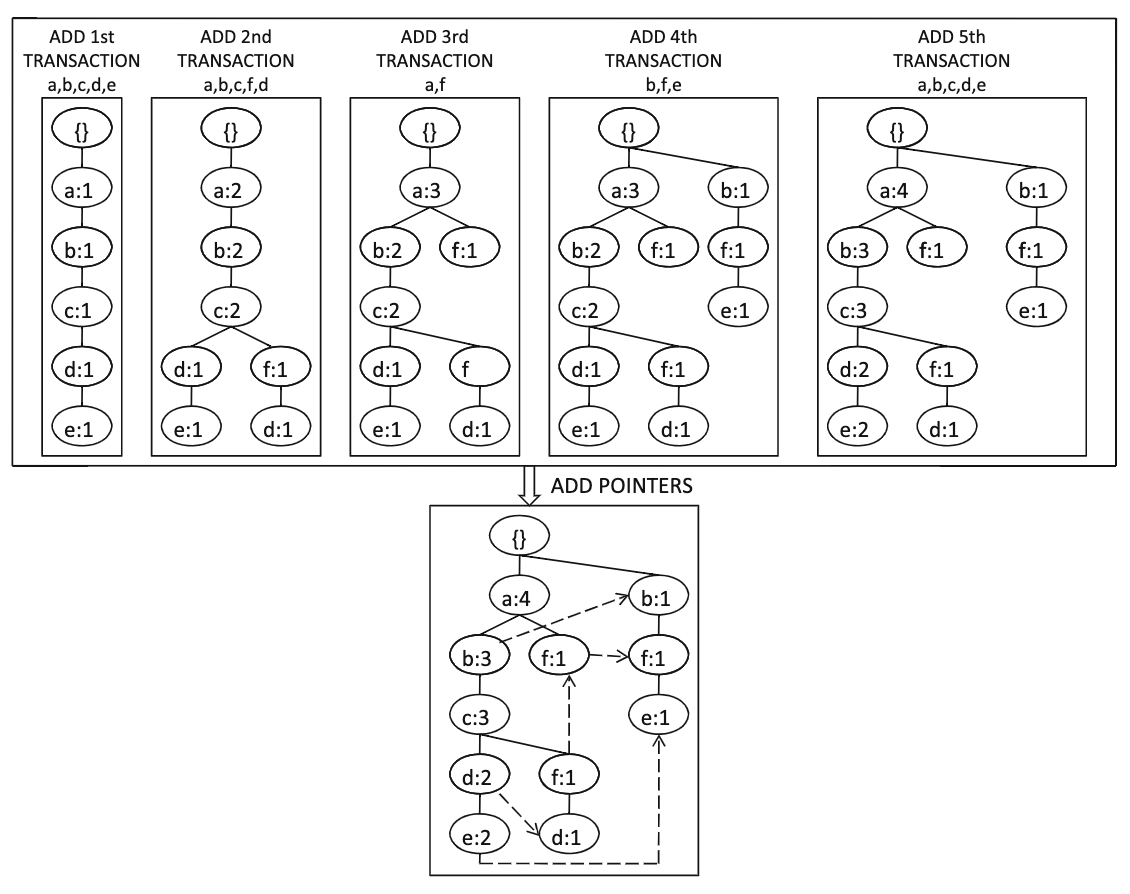
\includegraphics[width=1.0\textwidth]{RelatedWorks/fptree.png}
    \caption{An example of FP-Tree \cite{survey2014}}
    \label{fig:fp}
\end{figure}

When the situation becomes data stream mining, which means the data volume gets incredibly large, FP-Tree becomes very computational costly in both run time and space complexity. There are many existing researches \cite{fpopt1, fpopt2, fpopt3, fpopt4, fpopt5, fpopt6} focusing on tackling these issues. Most of the optimisations can be divided into two categories, one is using an advanced data structure to improve the performance like using arrays \cite{fpopt3}, another one holds partitioned database in the memory, for instance, CFP-Tree \cite{fpopt6}. Next, we are going to briefly discuss these two different mechanisms.

\begin{definition}[\textbf{\textit{CFP-Tree}}]
\label{ctpro}
Compact FP-Tree (CFP-Tree) was proposed by Sucahyo and Gopalan in 2004 \cite{fpopt6}. CFP-Tree is able to save the same amount information of FP-Tree but consumes 50\% memory. CFP-Tree does not have nodes that contains item label and support value, it maps item labels into index of thee head table - a sequence of integers. CPF-Tree accumulates duplicated sub-trees and keeps details in the leftmost branch, which achieves the compression of FP-Tree. 
\end{definition}

As FP-Tree constructs many conditional trees during the expansion, when the support value gets very low or association rule gets very long, it may gets beyond the system's affordability. CT-PRO algorithm solves this problem by adopting a non-recursive procedure. CT-PRO divides database into different parts which individual will be treated as a sole CFP-Tree independently. This significantly saves the memory use of the mining process.

To save the time for FP-growth to traverse FP-Tree, Grahne and Zhu \cite{fpopt3} used an array-like structure to improve FP-Tree. There are usually two traversals in the procedure of conducting FP-Tree, all frequent items are found during the first traversal and initialise a FP-Tree at the same time by finishing its header table construction. Then followed by the second traversal which will build a new tree. Grahne and Zhu \cite{fpopt3} started with creating an array during the first FP-Tree was construction to keep the information without the first scan.

This technique works significantly well when the database is very sparse. Sparse database requires more time for traversal which is massively reduced by using an array-like structure.

After all the discussions we had on association rule mining techniques, we may still need to get a rough idea of how data streams look alike before mining rules out from them. There are many algorithms been developed to construct a synopsis for data streams. One of the most important tasks is to get the top frequent items out from data streams.  

\subsection{Lossy Counting}

Lossy Counting \cite{lossy} provides a simple and efficient approximation for data stream to identify all elements whose current frequency exceeds a support threshold.

\begin{enumerate}
    \item First, divide data stream into fixed-sized windows.
    \item Second, increment the frequency count of each item according to the new window values. After each window, decrement all counters by 1.
    \item Last, repeat and update counters and after each window, decrement all counters by 1.
\end{enumerate}

In the end, the most frequently items will ``survive''. Given a frequency threshold $f$, a tolerance error $e$, and total number of elements $N$, all items with more than $f\times N - e \times N$ frequency will be returned as result. The primary window size is determined by the error rate $e$: $1/e$, and the number of windows will be $\lceil N\times e \rceil$, the worst case we need $(1/e)\times log(e\times N)$ counters.

\begin{figure}[H]
    \centering
    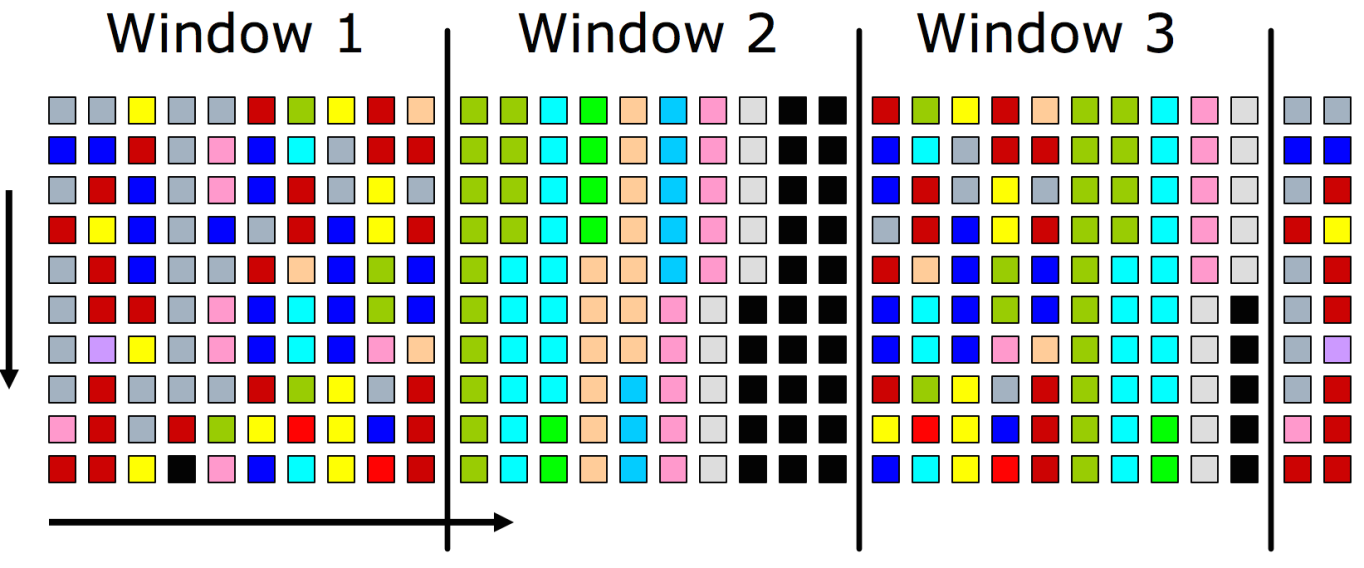
\includegraphics[width=0.8\textwidth]{RelatedWorks/lossy1.png}
    \caption{Step 1: divide windows \cite{lossymanku}}
    \label{fig:lossy1}
\end{figure}

\begin{figure}[H]
    \centering
    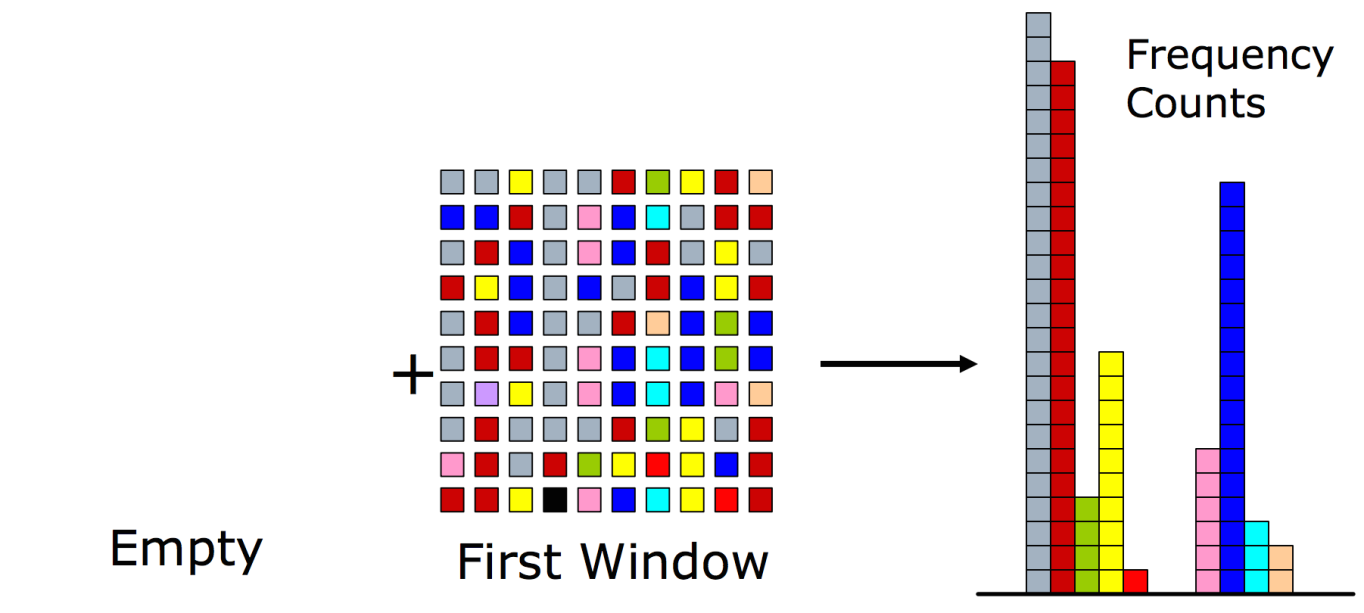
\includegraphics[width=0.8\textwidth]{RelatedWorks/lossy2.png}
    \caption{Step 2: increment counters \cite{lossymanku}}
    \label{fig:lossy2}
\end{figure}

\begin{figure}[H]
    \centering
    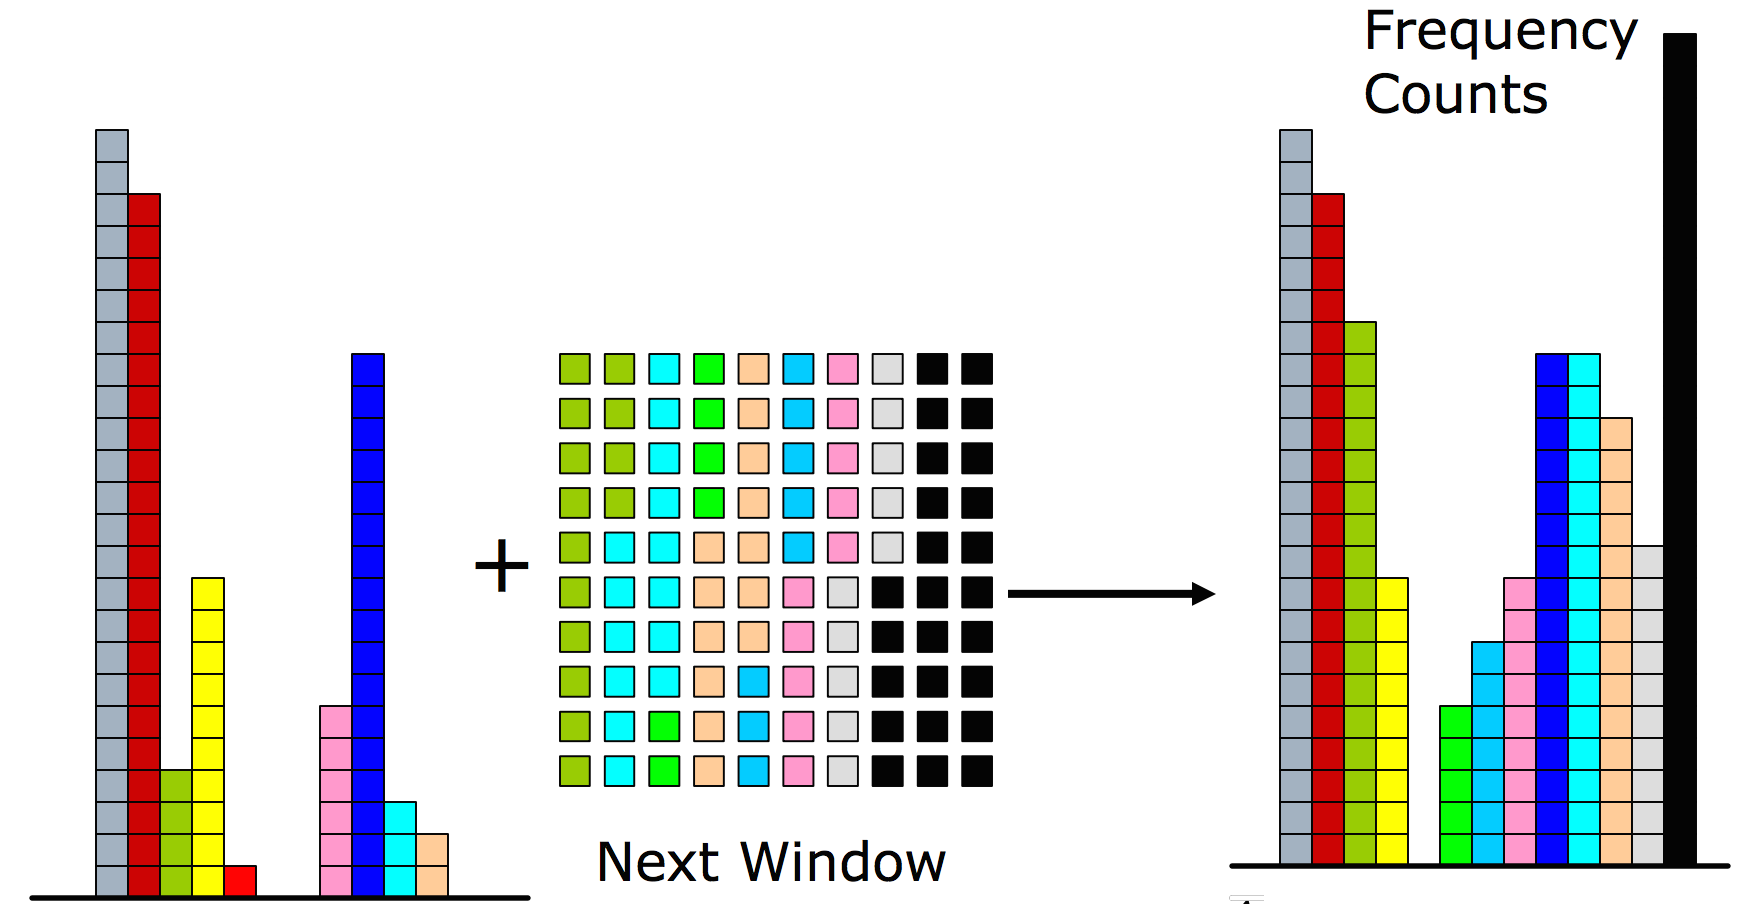
\includegraphics[width=0.8\textwidth]{RelatedWorks/lossy3.png}
    \caption{Step 3: decrement counters by 1 at boundary}
    \label{fig:lossy3}
\end{figure}



\subsection{Limitations of ``Support-Confidence” Framework}

Webb \cite{topk} pointed out that the traditional association rules mining techniques using minimum support and confidence threshold has numbers of limitations when apply them to most of the real-world scenarios.

First, there are some rare patterns which may be identified as frequent patterns by mistake. For instance, in the supermarket basket scenario, some terms may appear to be frequent but in fact, customers may act behalf of their company or friends which potentially lead to misclassifications.

Also, minimum support technique is relevantly a crude mechanism. It is almost impossible to pre-set a perfect minimum support threshold in advance, before the whole data stream is being analysed. Finding an appropriate threshold is usually tricky and sometimes leads to errors.

Dense data cannot be analysed by minimum support technique. It works fine when the terms in each transaction being relevantly infrequent. If numbers of terms appear frequently in each transaction, then the algorithm will produce a large number of interesting associations which is obviously wrong.

One of the most important, minimum support cannot be set low enough to
capture all valid rules. Nor can it be set high enough to exclude all spurious rules. Generally, minimum support may be irrelevant to the interestingness of associations.

\section{Concept Drift Mining} \label{sec:2.3}
This chapter focuses on concept drift detection, starts with definitions and types of concept drifts. Different kinds of drift detectors will also be discussed.

\subsection{Concept Drift}
Due to the inherent temporal aspect of data streams, the underlying data distribution of streams may change over time, known as concept drifts. Concept drift can make the machine learning model inaccurate because of the inconsistency between existing data and new data.

A transactional data stream $\mathcal{D}$ with $n$ elements $\mathcal{D} = \{T_1, T_2, ..., T_n\}$ where by $T_i$ represents a transaction at time $i$. At the time point $t$, let \mathcal{D}_1=(T_1, T_2, ..., T_t)$, $\mathcal{D}_2=(T_t_+_1, T_t_+_2, ..., T_n)$ be two instance of $\mathcal{D}$, with $0<t<n$ and their mean $\mu_1$ and $\mu_2$ respectively.

\begin{definition}[\textbf{\textit{Concept Drift Detection Problem}}]
\label{conceptdrift}
The concept drift detection problem is a statistical hypothesis test with the null hypothesis $H_0$ that $\mu_1=\mu_2$ and the alternative hypothesis $H_A$, that is, $\mu_1\neq\mu_2$.
\end{definition}

If the two samples $\mathcal{D}_1$ and $\mathcal{D}_2$ are drawn from the same distribution, the null hypothesis $H_0$ is justified, otherwise, the alternative hypothesis $H_A$ is accepted, a concept drift has been detected at the time point $t+1$. The position of this certain time point is also called \textit{drift point}.

In the data stream mining task, a concept drift may occur in different forms. In the next section, we review the types of concept drifts that can occur during data streams.

\subsection{Types of Concept Drifts}
Concept drifts can happen in different forms, there are two common types of drifts: abrupt drift and gradual drift.

\begin{definition}[\textbf{\textit{Abrupt Drift}}]
\label{abruptdrift}
An abrupt drift happens when there is a change in underlying distribution occurs instantaneously. Once an abrupt drift is detected, it usually means the whole distribution will remain changed after that point. 
\end{definition}
The figure below illustrates a simple example of an abrupt drift.

\begin{figure}[h!]
    \centering
    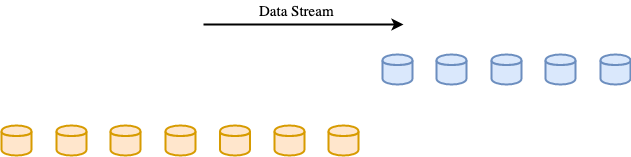
\includegraphics[width=0.7\textwidth]{RelatedWorks/abrupt.png}
    \caption{An example of abrupt drift}
    \label{fig:abrupt}
\end{figure}

%\paragraph{Gradual drift}\mbox{}\\

\begin{definition}[\textbf{\textit{Gradual Drift}}]
\label{gradualdrift}
Gradual drift, also known as incremental drift, is different from an abrupt drift. While abrupt change is caused by distribution changes instantaneously, gradual drift happens incrementally. This means between a potential change happens and the whole distribution actually changes, the data stream may remain the similar distribution as original.
\end{definition}

A simple example of an gradual drift has been illustrated below.

\begin{figure}[h!]
    \centering
    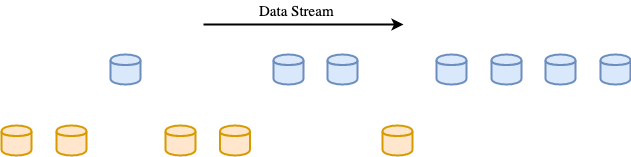
\includegraphics[width=0.7\textwidth]{RelatedWorks/gradual.png}
    \caption{An example of gradual drift}
    \label{fig:gradual}
\end{figure}

\subsection{Regional Concept Drift}%\mbox{}\\
Most distribution based drift detection methods assume that a drift occurs abruptly at a time point, incrementally, or gradually in a time period \cite{gradual}. As a result, the split time point between old and new concepts is the key solution. However, this time-oriented ``one-cut" process could not adapt to the real-world scenarios well. Accordingly, the data arrived before that drift point is discarded. Thus, if a drift only occurs in a small region of the entire feature space, the other non-drifted regions may also be suspended, thereby reducing the learning efficiency of models. %To retrieve non-drifted information from suspended historical data, similar to the buffer system \cite{buffer} used to find the best drift time point to identify concepts, we proposed a simple solution to identify regional drifts and integrate it into our self-sufficient itemset mining process.

\begin{figure}[h!]
    \centering
    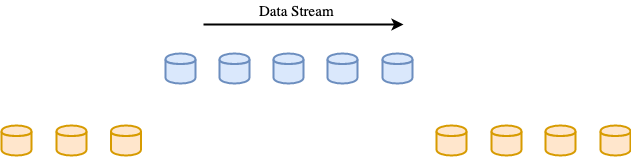
\includegraphics[width=0.7\textwidth]{RelatedWorks/regional.png}
    \caption{An example of regional drift}
    \label{fig:gradual}
\end{figure}

\subsection{Drift Detectors}

%\paragraph{DDM}\mbox{}\\

\begin{definition}[\textbf{\textit{DDM}}]
\label{ddm}
Drift Detection Method (DDM) is one of the earliest proposed drift detectors. DDM was built based on the PAC learning model premise, it assumes that the error rate decreases with more examples when the distribution is stationary.
\end{definition}

DDM analyses the error rate and some statistics such as standard deviation. There are normally two preset threshold: change and warning. When DDM detects an increase in the error rate and it surpasses the change threshold, a drift will be detected and reported. If the increase does not surpass the change threshold but the warning threshold, DDM will report a warning zone which indicates there might be changes happening in the near future.

%\paragraph{EDDM}\mbox{}\\
\begin{definition}[\textbf{\textit{EDDM}}]
\label{eddm}
%Drift Detection Method (DDM) has been proved useful for abrupt change detection. 
To improve the accuracy of detecting gradual changes in data stream, Early Drift Detection Method (EDDM) was proposed by keeping track of the average distance between two errors instead of only the error rate. 
\end{definition}

Similar to DMM, EDDM also has warning and change thresholds which are used for determine change levels.

%\paragraph{Page Hinkley}\mbox{}\\
\begin{definition}[\textbf{\textit{Page Hinkley}}]
\label{ph}

Page Hinkley \cite{PHT} method works by computing the observed values and their mean up to the current moment. 
\end{definition}

Page Hinkley won't output warning zone warnings, only change detection. The method works by means of the Page Hinkley test. Page Hinkley Test works as a sequential analysis mechanism which is often used as a concept drift detector. In general lines it will detect a concept drift if the observed mean at some instant is greater then a threshold value lambda \cite{PHT}.

%\paragraph{ADWIN}\mbox{}\\
\begin{definition}[\textbf{\textit{ADWIN}}]
\label{adwin}
ADWIN stands for ADaptive WINdowing, is an adaptive sliding window algorithm for detecting change, and keeping updated statistics about a data stream. 
\end{definition}

ADWIN decides the size of the window by cutting the statistics' window at different points and analysing the average of some statistic over these two windows. If the absolute value of the difference between the two averages surpasses a pre-defined threshold, change is detected at that point and all data before that time is discarded. 

ADWIN guarantees rigorous performance, by bounding its false positive and negative rates, which makes it an ideal solution for high-precision required situations.


\section{Self-Sufficient Itemsets} \label{sec:2.4}
While there are large amounts of literature on identifying and discovering association rules \cite{arm1,arm2,arm3,arm4}), they are all heavily reliant on using a support threshold to derive interesting association rules. The existing literature on identifying and discovering interesting rules beyond using support or frequency of occurrence is relatively sparse. Webb~\cite{patternwebb} points out that many pattern mining algorithms suffer from type-I errors which usually identifies infrequent itemsets as frequent. To deal with the drawbacks of the pure ``support-confidence" framework for pattern mining, Hamalainen \cite{kingfisher} proposed a solution which handles non-monotonicity. It also prunes redundant rules on-line. The quality of rules is estimated by the Fisher's exact test. `Self-sufficient itemsets" \cite{ssi} were created to solve this dilemma by contributing a set of constraints and statistical tests that can be applied during and after itemset discovery to identify itemsets whose frequency cannot be explained solely by either higher or lower-order interactions between factors within the data.

To improve the pure ``support-confidence” framework, Webb \cite{ssi} defined self-sufficient itemsets, which proposed \textit{itemset leverage}. \emph{Itemset leverage} is a measure for the degree of potential interest that arises naturally from the tests developed in \cite{ssi} by checking their productivity and non-redundancy. We further adapted the method by using Fisher's exact test to check for the minimum support threshold as well. This has been used in previous techniques \cite{kingfisher,ssi}.%[].

To be self-sufficient, an itemset must be \textit{productive}, \textit{non-redundant} and \textit{independently productive}.

Firstly, we introduce the definition of cover, similar to support, which helps us understand how self-sufficient itemset.

\begin{definition}[\textbf{\textit{Cover}}]
\label{df:cover}
The \textit{cover} of an itemset $x$ is the set of TIDs which contains $x$:
\end{definition}

\begin{equation}
\label{eq:cover}
cov(x, \mathcal{D}) = \{i: 1\leq i\leq |\mathcal{D}| \wedge x \subseteq \mathcal{D}_i\}
\end{equation}

\begin{definition}[\textbf{\textit{Fisher's exact test}}]
\label{df:fishers}
Fisher's exact test is the main statistical test used to define self-sufficient itemset. It is a statistical test used to determine if there are nonrandom associations between two categorical variables.

Let there exist two such variables $X$ and $Y$, with $m$ and $n$ observed states, respectively. Now form an $m\times n$ matrix in which the entries $a_i_j$ represent the number of observations in which $x = i$ and $y = j$. Calculate the row and column sums $R_i$ and $C_j$, respectively, and the total sum: 

\begin{equation}
\label{eq:fisherssum}
N = \sum_{i} R_i = \sum_{j} C_j
\end{equation}

of the matrix. Then calculate the conditional probability of getting the actual matrix given the particular row and column sums, given by:

\begin{equation}
\label{eq:fishersformula}
P_{cutoff}=\frac{(R_1! R_2! \cdots R_m!)(C_1! C_2! \cdots C_n!)}{N!\prod_{i,j} a_{ij}!}
\end{equation}

which is a multivariate generalisation of the hyper-geometric probability function. Now find all possible matrices of non-negative integers consistent with the row and column sums $R_i$ and $C_j$. For each one, calculate the associated conditional probability using Eq. \ref{eq:fishersformula}, where the sum of these probabilities must be 1.
\end{definition}


\begin{definition}[\textbf{\textit{Productivity}}]
\label{df:productivity}
An itemset has to satisfy the following condition to be self-sufficient: any partition of it into two subsets of terms must be positively correlated with each other.

\begin{equation}
\label{productive}
P(R \supseteq x) >  \underset{y \subsetneq x}{max}(P(R \supseteq y)P(R \supseteq x \setminus y))
\end{equation}

It is hard to obtain the probabilities which leads us to perform a statistical test. In this case, Fisher's Exact Test is being used. The $p$-value for the case whether itemset $x$ and $y$ of dataset $D$ are positively correlated should look like this:

\begin{equation}
\label{fishersp}
p_{F}(x, y, D) = \sum_{i=0}^{\omega} \frac{\binom{\#(x, D)}{\#(x, y, D)+i}\binom{\#(\neg x, D)}{\#(\neg x, y, D)+i}}{\binom{n}{\#(y, D)}}
\end{equation}

where $\omega$ = min($\#(x,\neg y, D), \#(\neg x, \neg y, D)$). \cite{ssi}

To test productivity for an itemset $m$ , all of its partitions need to be passed the Fisher's test.

\begin{equation}
\label{fisherspartition}
p(m,D) = \underset{x \subsetneq m}{max}(p(x, m \setminus x, D))
\end{equation}


\end{definition}


\begin{definition}[\textbf{\textit{Redundancy}}]
\label{df:redundancy}
Redundancy test provides another criteria to filter itemsets that are unlikely to be interesting. If an itemset $x$ has a subset $y$ which contains an item $i$ that subsumes $y\setminus i$, we define $x$ as redundant. This has also been discussed for constraints of association rule mining. \cite{redundant}

\begin{equation}
\label{eq:redundant}
\exists i, y : i\in y \wedge y \subsetneq x \wedge cov(\{i\}) \supseteq cov(y \setminus i)
\end{equation}

\end{definition}


\begin{definition}[\textbf{\textit{Independent Productivity}}]
\label{df:indprod}
In terms of quantifying interestingness, the Min Partition Measure (MPM) is used. Webb \cite{ssi} suggests that itemset measures should be developed from a rule measure by selecting the least extreme value that results from applying the measure to any rule that can be created by partitioning the itemset $x$ into an antecedent $y$ and consequent $z = x \setminus y$. In this work, two measures: $leverage, \delta$ and $lift, \gamma$ have been used as the formulas Eq. \ref{eq:leverage} and Eq. \ref{eq:lift} illustrated below:

\begin{equation}
\label{eq:leverage}
\delta(x) = \underset{y \subsetneq x}{min}(sup(x)-sup(y)\times sup(x \setminus y))
\end{equation}

\begin{equation}
\label{eq:lift}
\gamma(x) = \underset{y \subsetneq x}{min}(sup(x)/ [sup(y)\times sup(x \setminus y)])
\end{equation}

\end{definition}

\subsection{OPUSMiner}
OPUSMiner~\cite{patternwebb} is developed to find the top-$k$ productive, non-redundant itemsets from transaction data. The OPUS Miner algorithm uses the OPUS search algorithm to efficiently discover the key associations in transaction data, in the form of self-sufficient itemsets, using either $leverage, \delta$ as in Eq. \ref{eq:leverage} or $lift, \gamma$ as in Eq. \ref{eq:lift}.

OPUSMiner is conducted with four parts: expandItemset, checkPartitions, checkImmediateSubsets and checkIndeproductive. Each part will achive the cooresponding task which is a compulsory condition for an itemset to be self-sufficient.

\begin{enumerate}
    \item expandItemset: explore all supersets of a generated itemset $X$ from beginning by adding items in the frequent item list $q$.
    \item checkPartitions: check the binary partitions of itemset $X$. Return the minimum value of $\delta $ and $ \gamma$ and the maximum $p$-value $p$ with respect to any partition.
    \item checkImmediateSubsets: check all subsets of $X$ formed by removing a single item to determine whether $X$ fails the Apriori test and whether supersets of $X$ must fail either the Apriori or redundancy test.
    \item checkIndeproductive: post-process the top $k$ itemsets to determine whether they are independently-productive.
\end{enumerate}

OPUS Miner systematically traverses viable regions of the search space, maintaining a collection of the top-$k$ productive non-redundant itemsets in the search space explored. When all of the viable regions have been explored, the top-$k$ productive non-redundant itemsets in the search space explored must be the top-$k$ for the entire search space.

\subsection{Concept Drifts in Self-Sufficient Itemsets Mining}

According to \cite{classsurvey}, an important problem in the streaming scenario is classification, where data is labelled into categories or classes. As data streams are considered to be non-stationary, the distribution of data and their class labels will likely change over time. Concept drift detection methods are used to monitor classification errors from classifiers (with binary input where 0 is a correct classification and 1 is a misclassification) to identify when changes happen. In our scenario, we want to determine how frequent potential ‘interesting’ itemsets occur in the data stream. The measure we used to feed our drift detector with will be the binary occurrence of itemsets in each transaction of the data stream (0 if itemset is not present and 1 if itemset is present). Gama et al. \cite{driftsurvey} gives an overview of mainstream drift detectors used for data stream. One of the most widely used detector is ADWIN \cite{adwin}. ADWIN detects concept drifts using an adaptive windowing strategy and signals drifts if the absolute value of the difference between any two windows surpasses a pre-defined threshold, derived from Hoeffding Bound.

\section{Summary of Literature} \label{sec:2.5}

There are many researches focusing on the field of association rule mining and concept drift mining. We reviewed the research problems and studies their proposed solutions and methodologies.

In association rule mining, the major problem is to discover significant patterns out from unlabelled item based data which usually comes in a form of transaction, as known as transactional data stream using unsupervised machine learning techniques. Traditional ``support-confidence'' framework like Apriori \cite{apriori} and FP-growth \cite{fp} has been adopted to solve most of the association rule mining problems in the past decades, its drawbacks has become an issue for association rule mining. We reviewed several new association rule mining algorithms proposed to solve these drawbacks such as improving the adaptability of support threshold \cite{armlin}, adding statistical tests to filter rules \cite{kingfisher} and defining new restraints to create association rules \cite{topk,ssi}. 

Concept drift mining focuses on detecting the underlying distribution change and adapting to the drifts detected. Drifts have different types such as abrupt, gradual and regional drifts. The difference between abrupt and gradual drifts is the time they occur: abrupt drifts only happen in a very short period or time while gradual drifts may need longer period. Regional drifts are those drifts which occur during a specific period of time. Many concept drift detectors have been proposed to solve the problem, we have reviewed them in different categories in statistics control (e.g. EDDM and DDM), sequential analysis (e.g. Page Hinkley), and sliding-window monitoring (e.g. ADWIN).



